% Created by tikzDevice version 0.12.3.1 on 2022-01-16 03:37:54
% !TEX encoding = UTF-8 Unicode
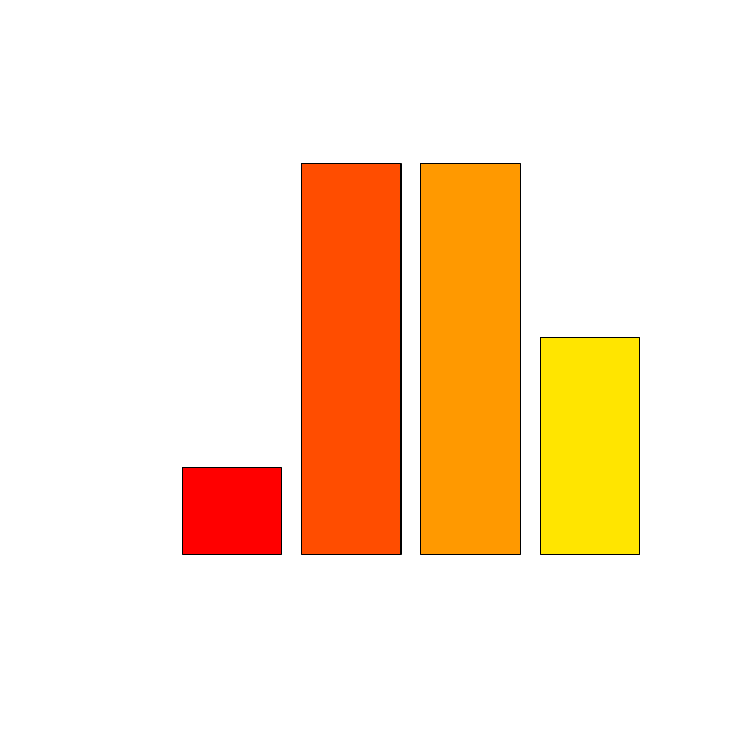
\begin{tikzpicture}[x=1pt,y=1pt]
\definecolor{fillColor}{RGB}{255,255,255}
\path[use as bounding box,fill=fillColor,fill opacity=0.00] (0,0) rectangle (252.94,252.94);
\begin{scope}
\path[clip] (  0.00,  0.00) rectangle (252.94,252.94);
\definecolor{drawColor}{RGB}{0,0,0}
\definecolor{fillColor}{RGB}{255,0,0}

\path[draw=drawColor,line width= 0.4pt,line join=round,line cap=round,fill=fillColor] ( 55.81, 62.61) rectangle ( 91.75, 93.97);
\definecolor{fillColor}{RGB}{255,77,0}

\path[draw=drawColor,line width= 0.4pt,line join=round,line cap=round,fill=fillColor] ( 98.94, 62.61) rectangle (134.88,203.75);
\definecolor{fillColor}{RGB}{255,153,0}

\path[draw=drawColor,line width= 0.4pt,line join=round,line cap=round,fill=fillColor] (142.07, 62.61) rectangle (178.01,203.75);
\definecolor{fillColor}{RGB}{255,229,0}

\path[draw=drawColor,line width= 0.4pt,line join=round,line cap=round,fill=fillColor] (185.19, 62.61) rectangle (221.13,141.02);
\end{scope}
\end{tikzpicture}
